\chapter{State of the Art - Cheats and Anti-Cheats}

\label{chap:one}

\epigraph{\itshape Technology is just a tool. In terms of getting the kids working together and motivating them, the teacher is the most important.}{-- Bill GATES}

\startcontents[chapters]

\printMyMinitoc

\fancyhead[LE]{\textsc{\chaptername~\thechapter}}

\section{Cheat-Based Exploration of System Architecture}
\label{sec:one:one}

\subsection{Automation Cheats}
\label{sec:one:one:one}

Automation cheats represent a critical class of malicious software engineered to augment or entirely substitute a player's mechanical execution within the competitive environment. This category primarily encompasses automated aiming tools (aimbots), automatic firing utilities (\glsps{triggerbot}), and execution macros or \glspl{script}. By targeting the core pillars of first-person shooter (FPS) gameplay—specifically mechanical precision, muscle memory, and cognitive reaction time, these tools disrupt competitive balance by replacing human motor control with software-driven operations.

To achieve this automation, the software must interface directly with either the operating system's input layer or manipulate the inner variables governing the game engine logic. The depth of this interaction generally defines the cheat's sophistication and detection difficulty:

\begin{itemize}
    \item Input Layer Manipulation: Client-side automation tools often operate by injecting synthetic mouse and keyboard events directly into the operating system's input stream. A typical triggerbot, for example, continuously polls the game client's state or memory addresses to determine when an enemy entity's hitbox intersects with the exact coordinates of the player's crosshair. The moment this condition is validated, the cheat programmatically fires a click event into the input queue, completely bypassing human visual processing and nervous system latency. The latency between the detection of the event and the actual input can be configured to try and pass as a human reaction, though the main point of this process is still to be way faster than the average player.
    \item Subversion of Game Engine Logic: More advanced automation mechanisms bypass peripheral input emulation altogether, executing modifications directly within the local game engine client memory space. An aimbot reads the real-time spatial positions (three-dimensional coordinates) of all active opponents from the engine's local entity list. It then calculates the precise angular vector offsets required to bridge the gap between the current viewpoint and the target's head hitbox. By overwriting the client's view-angle variables within the engine memory before the next frame rendering or \gls{tick} packet serialization, the cheat forces perfect accuracy.
\end{itemize}

\begin{figure}[!h]
    \begin{center}
        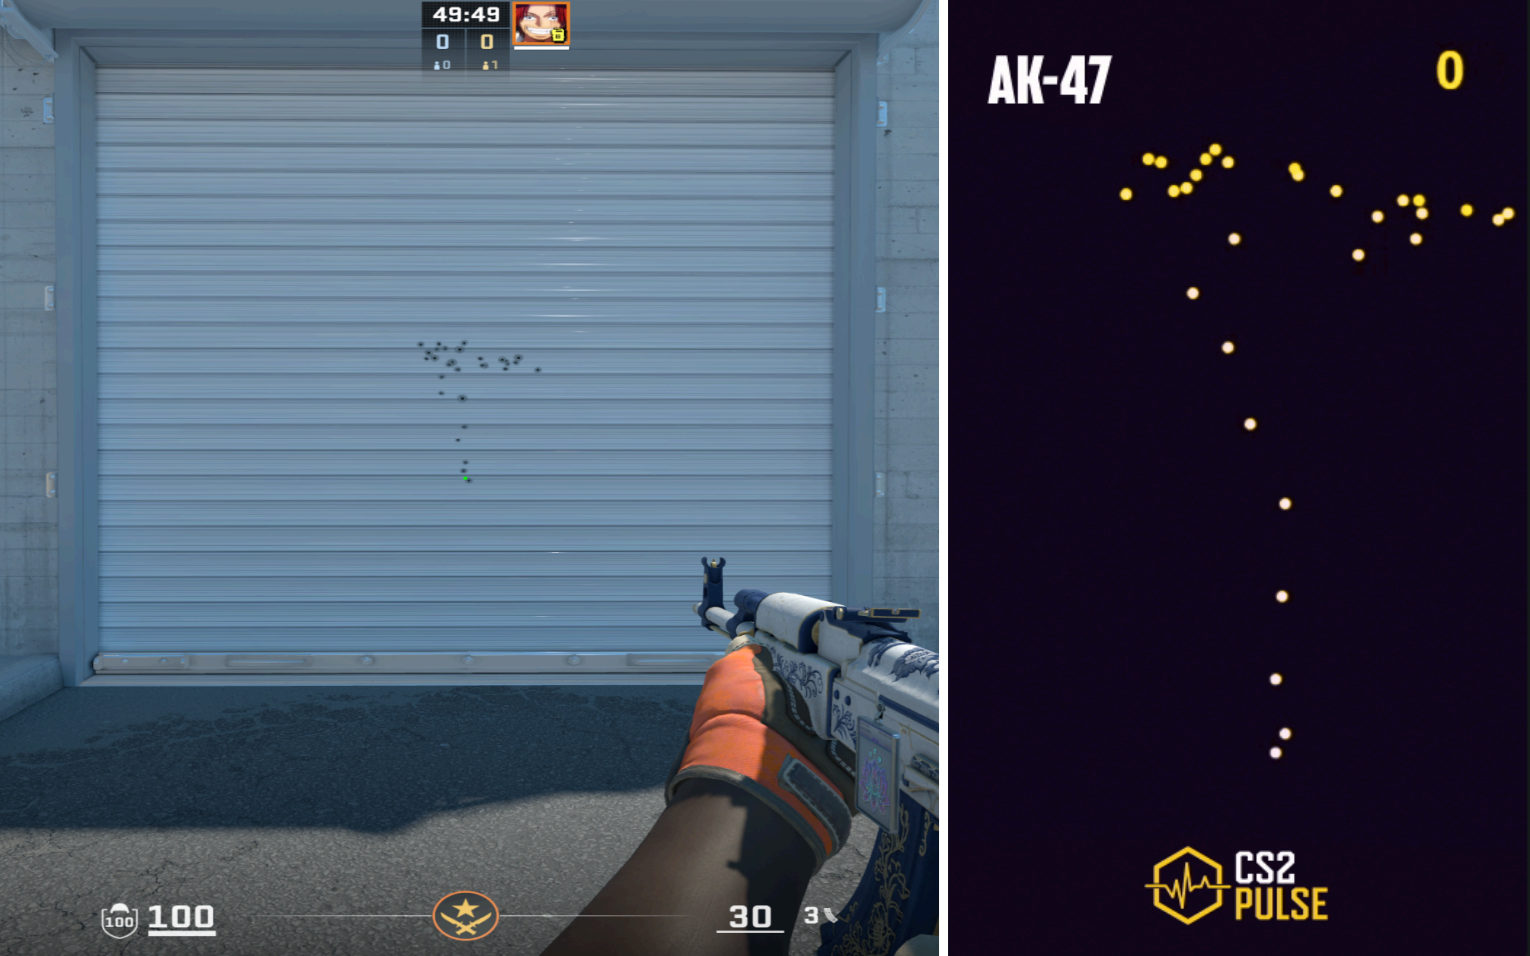
\includegraphics[height=9cm]{../images/chap01/fig1.png}
    \end{center}
    \caption[Comparison of the recoil from the AK-47 in-game with its theoretical model, implying that the recoil is deterministic and can be compensated for with a script.]{https://cs2pulse.com/spray-patterns/ak-47/}
    \label{fig:fig1}
\end{figure}

This enables frame-perfect recoil compensation and automated target tracking that completely overrides the physical constraints designed by the game developers, as illustrated in Figure 1, which confirms the deterministic nature of the AK-47's spray pattern and the trivial feasibility of scripted compensation.

\subsection{Information Cheats}
\label{sec:one:one:two}

Unlike automation tools that directly override a player's physical inputs, information cheats focus on subverting the tactical integrity of tactical shooter ecosystems by breaking down spatial boundaries. Tactical first-person shooters heavily rely on a conceptual "fog of war"—a structural design where information regarding enemy positions, utility placement, and movement is deliberately occluded by spatial geometry to reward map control and sensory awareness. Information cheats, primarily manifested as wallhacks and \glspl{radarhack}, systematically dismantle this baseline restriction. They do not execute actions for the user but instead grant an absolute cognitive advantage by exposing hidden game data and altering the rendering pipeline.

To achieve this asymmetric visualization, these tools typically exploit two distinct technical vectors within the local client system:

\begin{figure}[!h]
    \begin{center}
        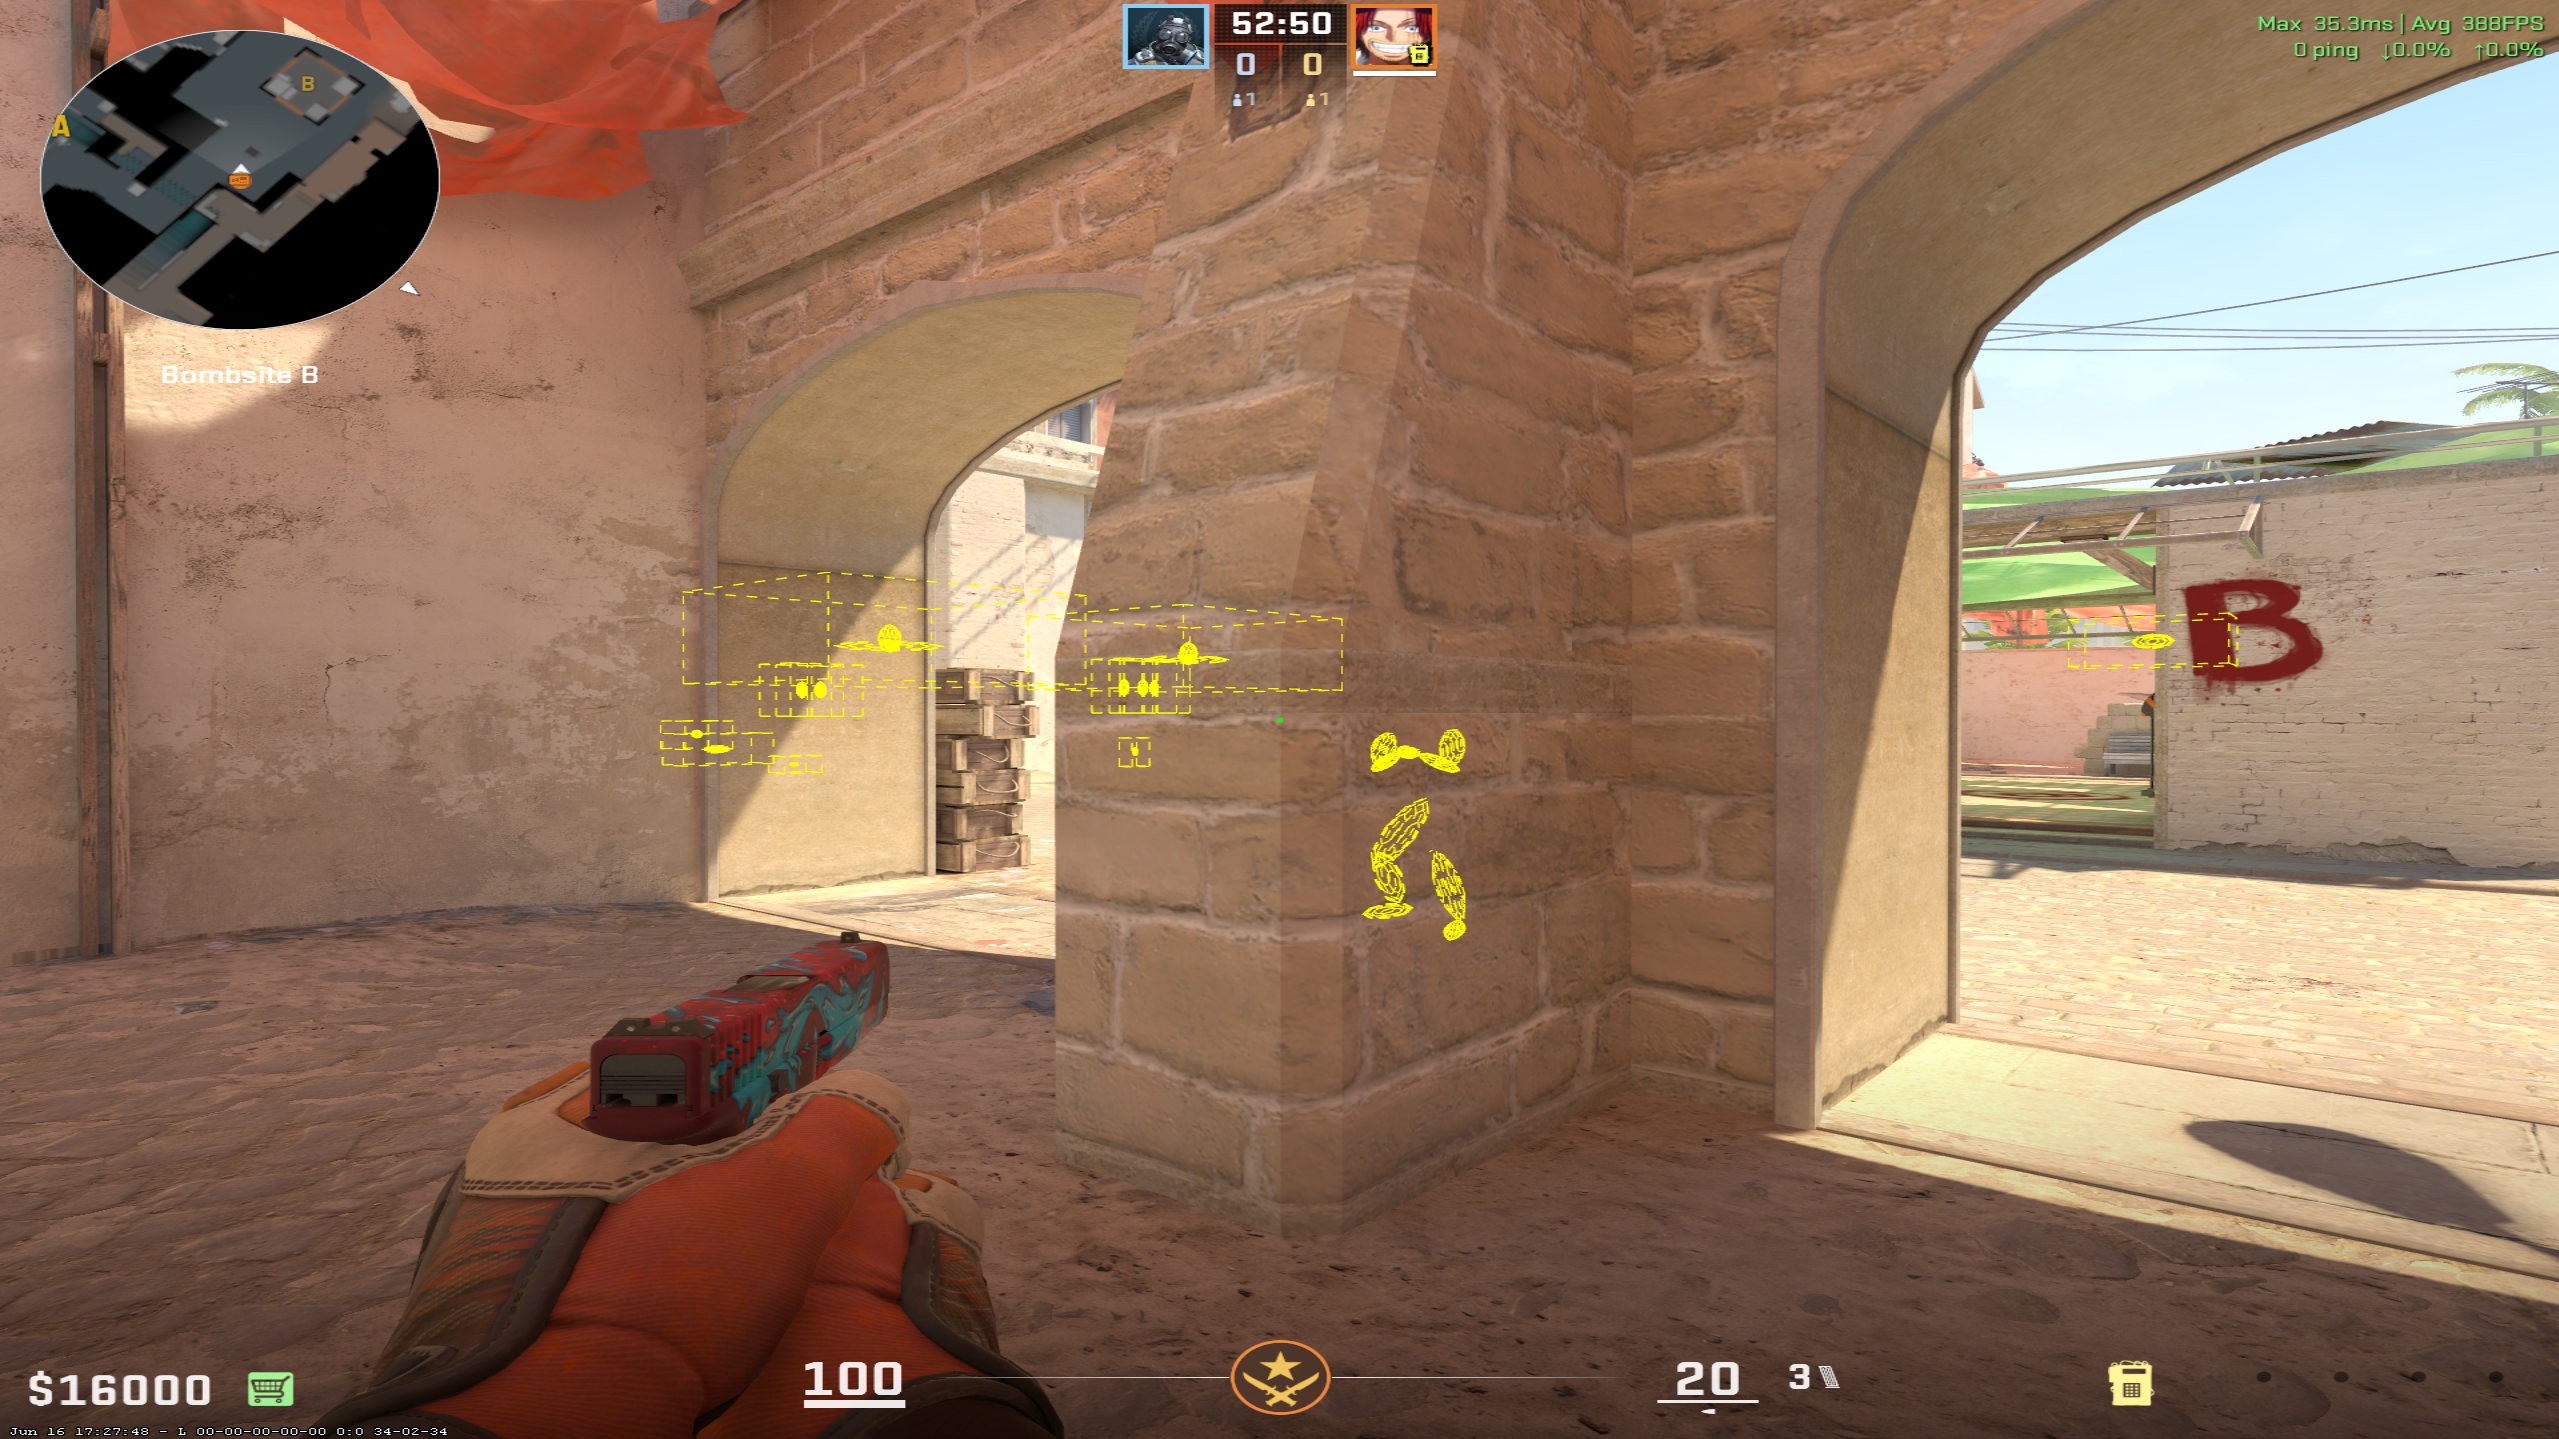
\includegraphics[height=9cm]{../images/chap01/ingamewallhack.png}
    \end{center}
    \begin{center}
        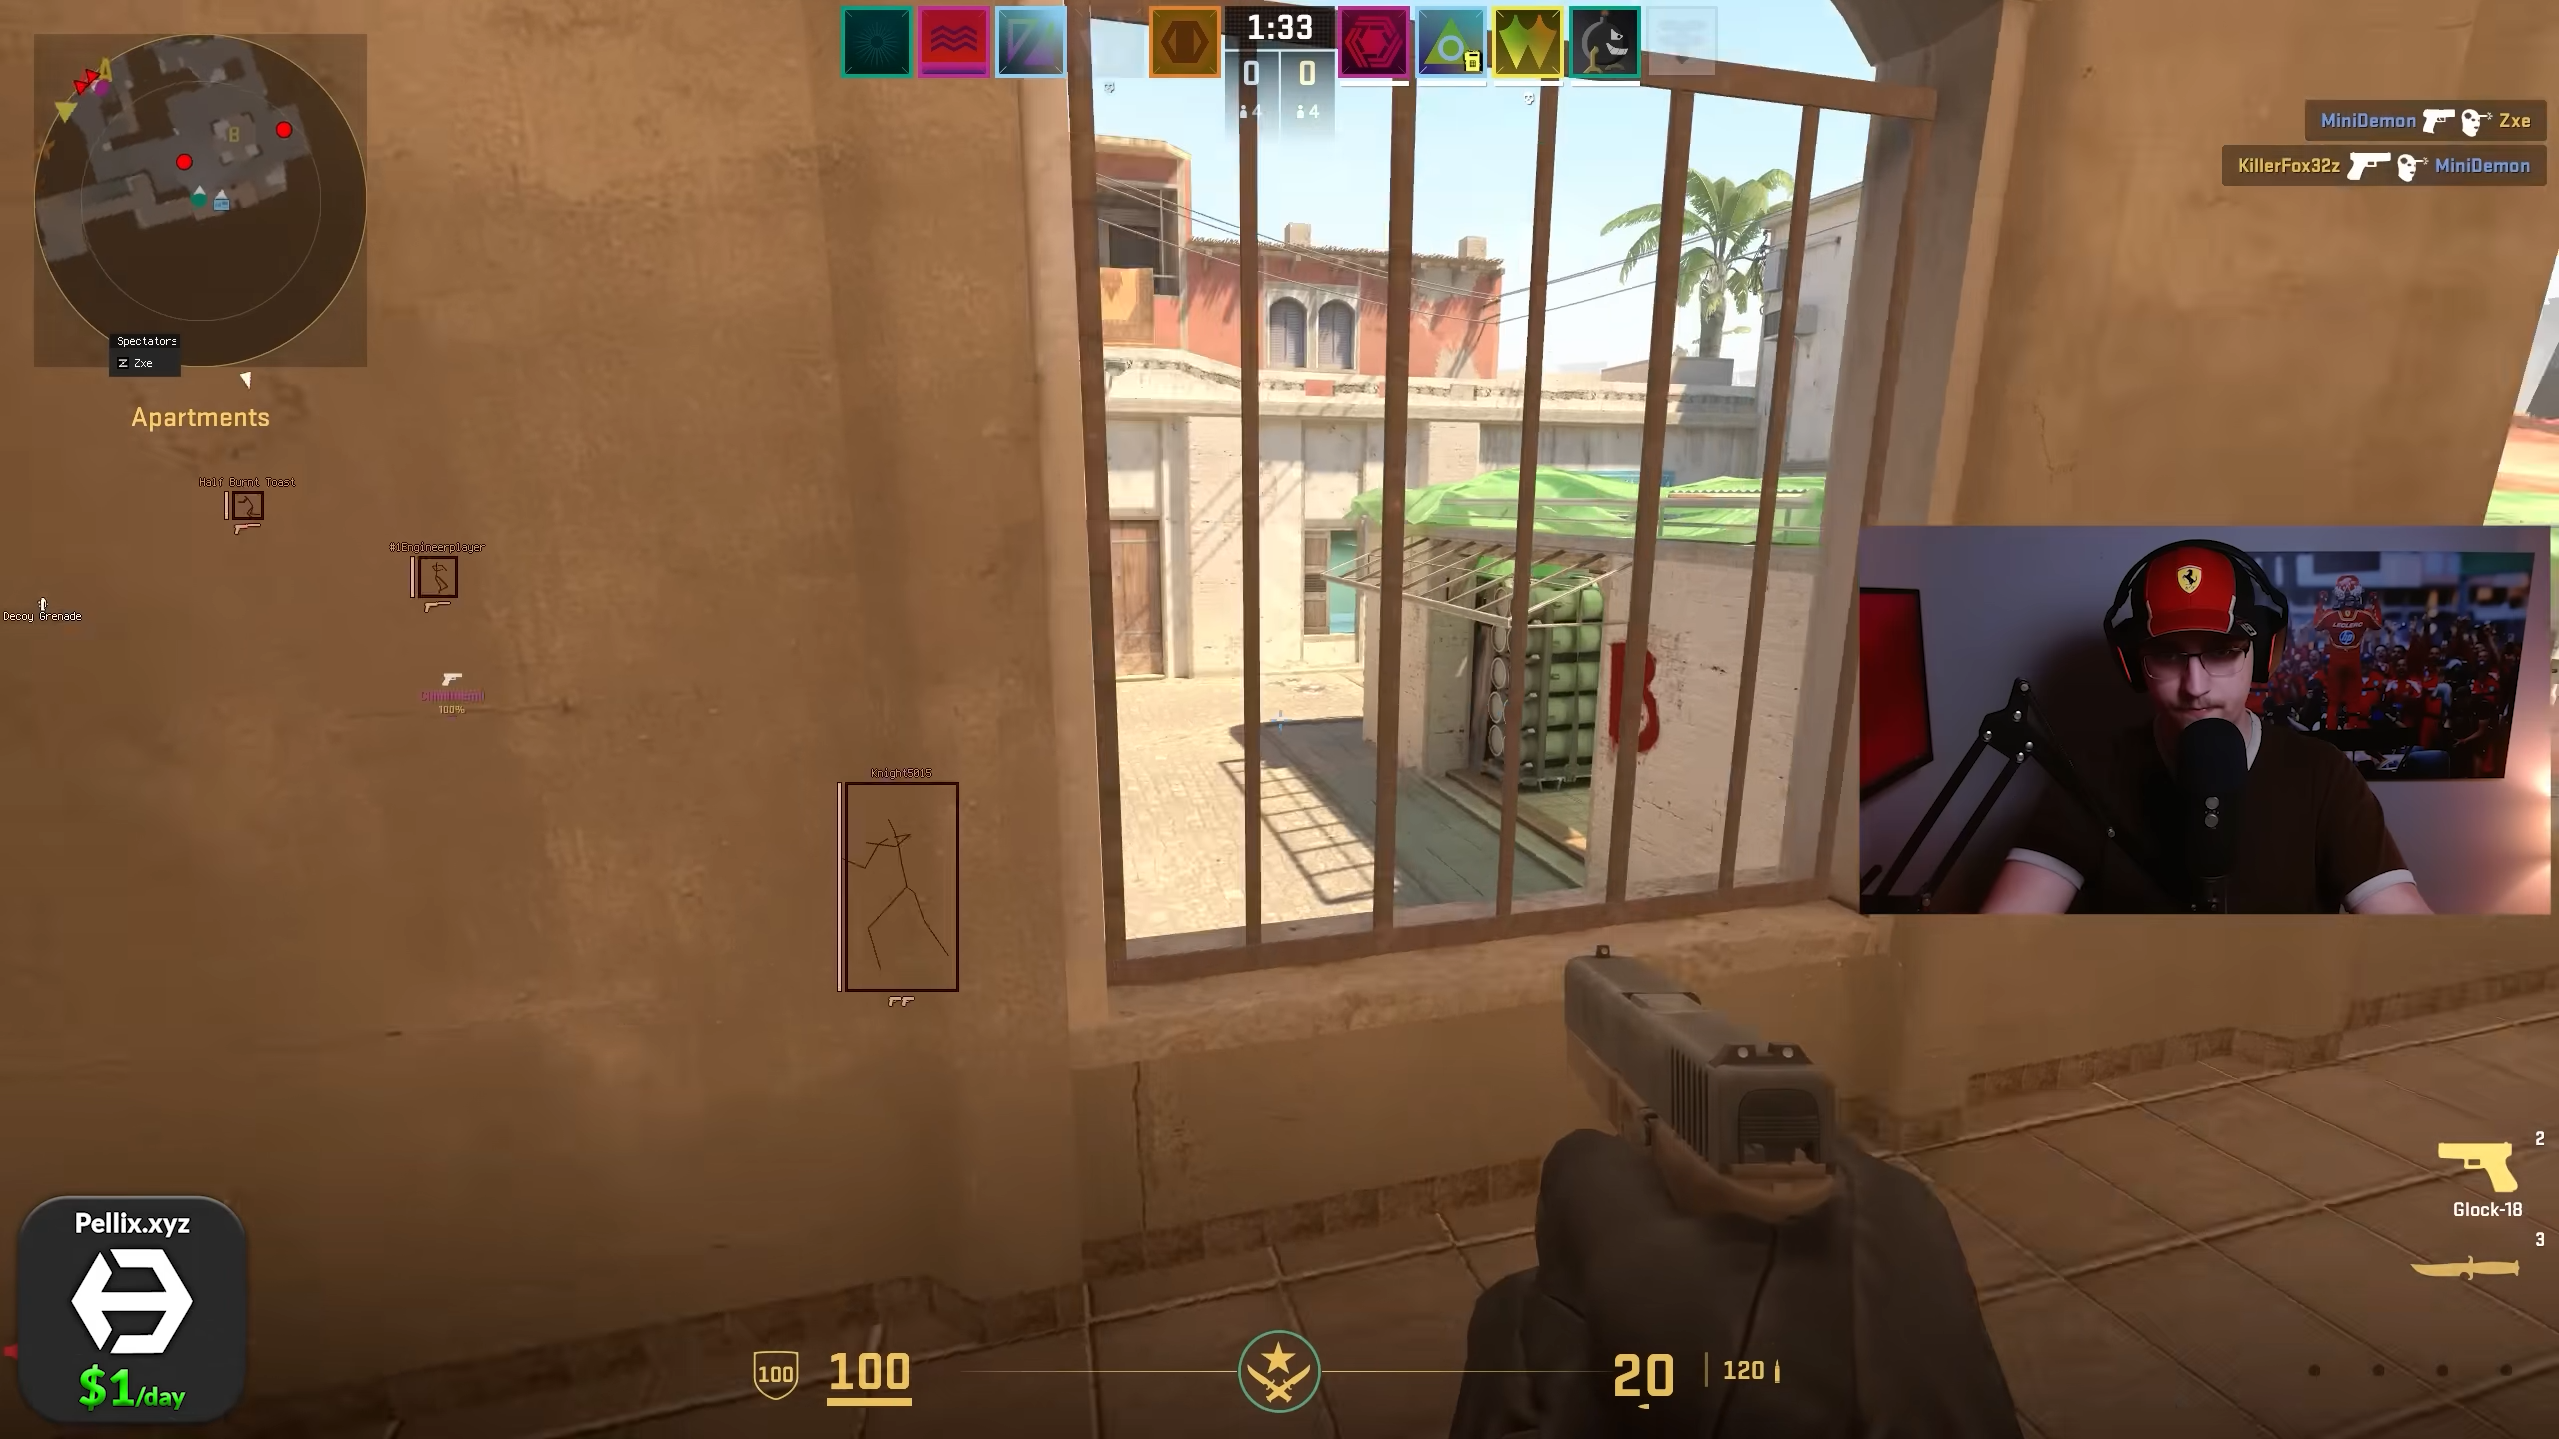
\includegraphics[height=9cm]{../images/chap01/paidwallhack.png}
    \end{center}
    \caption{Comparison of wallhack demonstration using built-in command "r\_aoproxy\_show 1" in CS2, which forces the engine to render near entity models regardless of occlusion (top) and an ad from a cheating software provider showing wallhack in action (bottom).}
    \label{fig:comparisonwallhack}
\end{figure}

\begin{itemize}
    \item Rendering Pipeline Exploitation: Wallhacks operate by intercepting or altering the graphics rendering pipeline responsible for drawing the game world onto the player's screen. In a legitimate game loop, the engine utilizes occlusion to ensure that player models hidden behind opaque geometry (such as walls or solid terrain) are not drawn on the screen. Wallhacks circumvent this by hooking into the graphic \gls{API}s (APIs) used by the engine. By injecting code that forces the graphics card to ignore occlusion parameters when processing enemy entity models, the cheat renders these entities on top of intervening geometry. This is frequently accompanied by \gls{ESP} (ESP) boxes, which overlay real-time lines, health bars, and item descriptions directly onto the player's view canvas — a result visually indistinguishable from the engine's own debug rendering mode, as shown in Figure 2, where the output of a native CS2 command forcing occlusion bypass (top) is compared side-by-side with a commercial cheat advertisement (bottom).

    \item Game Data Exposure: Radarhacks bypass the visual canvas entirely, targeting the underlying spatial data structures residing within the client’s volatile memory or network socket streams. Every online game client maintains a local "Entity List" containing the precise three-dimensional coordinate vectors of all active participants, transmitted by the server to ensure local interpolation and hit registration. A radarhack continuously scans the process memory space to extract these spatial vectors or sniffs incoming network packets before they are parsed by the client. This data is then projected onto a secondary web-based interface, an external execution window, or a simulated 2D mini-map overlay. Because this methodology leaves the primary visual interface completely clean and does not alter rendering hooks, it provides the cheater with absolute situational awareness while significantly minimizing visibility to automated anti-cheat screen capture mechanisms or human review systems. This type of cheating is one of the hardest to detect as, except for the direct scanning of the process memory space, the behaviour of such cheaters can often be associated with a good game-sense or instincts, hence being harder to prove as blatant cheating — Figure 3 illustrates this extraction pipeline, showing enemy coordinates pulled from the entity list and projected onto a clean secondary interface that leaves the primary game view entirely unaltered.
\end{itemize}

\begin{figure}[!h]
    \begin{center}
        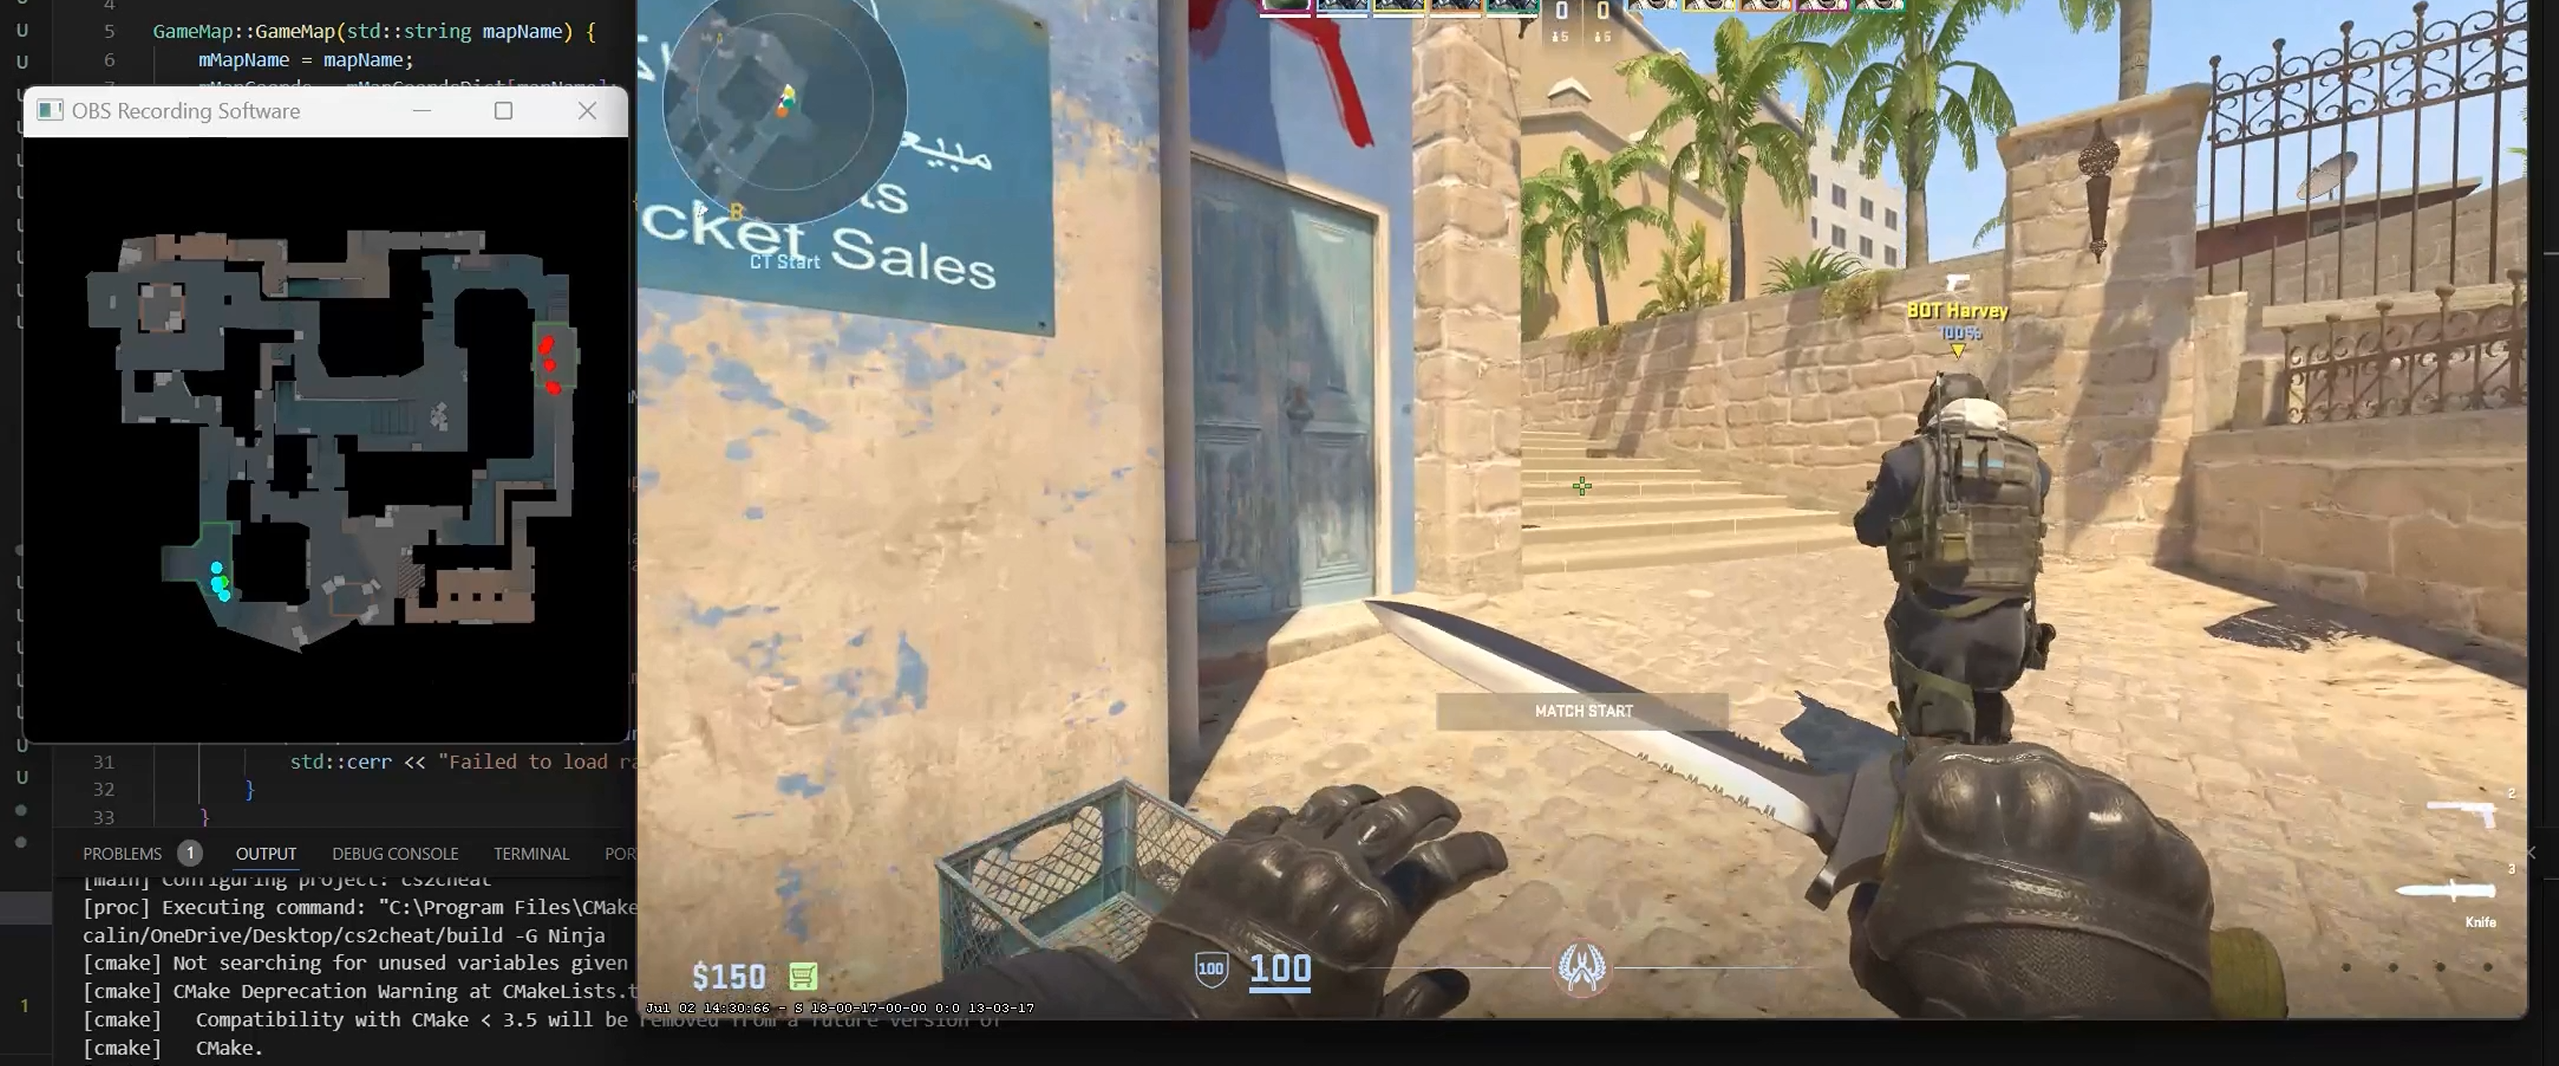
\includegraphics[height=7cm]{../images/chap01/radarhack.png}
    \end{center}
    \caption[Radarhack demonstration showing the extraction of enemy positions from the game's entity list and their projection onto a secondary interface.]{https://github.com/bordeanu05/cs2cheat}
    \label{fig:figradarhack}
\end{figure}

\subsection{Advanced Cheats}
\label{sec:one:one:three}

As client-side anti-cheat mechanisms evolved to actively monitor user-mode operations, the cheating ecosystem shifted toward highly sophisticated execution paradigms categorized as advanced cheats. These advanced threats deliberately bypass the operating system's standard application boundaries by executing within highly privileged environments or utilizing standalone external hardware vectors. By exploiting low-level OS/Kernel interactions and dedicated hardware interfaces, these tools minimize or entirely eliminate their local software footprint, rendering conventional user-mode memory scanners and API hooks ineffective.

\begin{figure}[!h]
    \begin{center}
        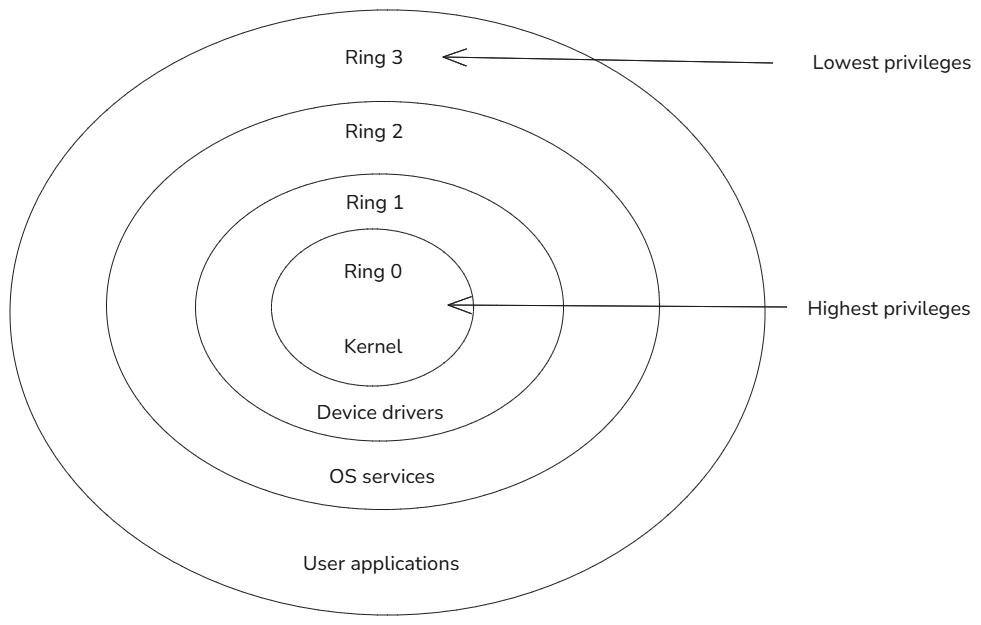
\includegraphics[height=9cm]{../images/chap01/fig4.png}
    \end{center}
    \caption[Privilege \gls{rings} in an OS' structure, highlighting the elevated access of kernel-level cheats in Ring 0 compared to user-mode applications in Ring 3.]{https://www.tutorialspoint.com/article/protection-ring}
    \label{fig:fig4}
\end{figure}

\begin{itemize}
    \item Kernel-Level Cheats and Kernel interaction: Kernel-level cheats operate inside the most privileged layer of the computer's processor architecture, known as Kernel Mode (Ring 0). While regular video games and applications are restricted to User Mode (Ring 3) where they have limited permissions, software running in Ring 0 has absolute control over the entire system's memory and hardware. Because modern client-side anti-cheat systems also run at this kernel level to monitor the game, cheat developers must find ways to gain equal authority to hide their presence and subvert security controls — a dynamic directly reflected in the privilege ring architecture shown in Figure 4, where both kernel-level cheats and anti-cheats compete for the same Ring 0 authority, leaving user-mode applications in Ring 3 with no visibility over either.

    This advanced interaction with the operating system occurs through two primary mechanisms:

    \begin{itemize}
        \item System Penetration via \gls{BYOVD} (BYOVD): Modern operating systems like Windows require all kernel-level software to be digitally signed and approved by \gls{Microsoft}. To bypass this security check, cheat developers use a technique called Bring Your Own Vulnerable Driver (BYOVD). They take an old, legitimately signed utility driver (from a trusted company) that contains a known security flaw. The cheat loads this trusted driver into the system and exploits its vulnerability to inject unsigned, malicious cheat code directly into the secure kernel memory space.
        \item Direct System Manipulation: Once established inside Ring 0, the cheat can modify the operating system's internal tracking structures. Using a method known as  \gls{DKOM} (DKOM), the cheat can erase its own program from the active process list or alter the system’s memory maps. This disguises the cheat's memory footprint, making it look like a harmless, native operating system component.
    \end{itemize}

    \item External Cheats and Hardware Interfaces: The most modern escalation in this technical conflict involves external and hardware-assisted cheats, which decouple the cheat execution environment from the host operating system running the game client. This paradigm relies on physical hardware interfaces, most notably Direct Memory Access (DMA) via specialized hardware expansion cards installed directly into the host machine's \gls{PCIe} (PCIs) slots. The DMA card physically reads and writes to the system's volatile \gls{RAM} (RAM) directly through the hardware controller, completely bypassing the \gls{CPU} (CPU) and any software-level security controls enforced by the operating system kernel. This raw memory stream is transmitted via a physical interface to a secondary, completely isolated computer. This external machine parses the game state asynchronously,calculates visual overlays or aim vectors, and can send synthetic peripheral inputs back to the host via specialized hardware input spoofers or modified mouse firmware. Because no malicious code executes, modifies memory, or hooks processes on the primary gaming machine, hardware-assisted vectors leave zero software footprint for traditional detection engines to scan — Figure 5 details this infrastructure, showing how the PCIe card reads host RAM through the hardware controller and relays the raw memory stream to an isolated external machine responsible for processing and input spoofing.
\end{itemize}

\begin{figure}[!h]
    \begin{center}
        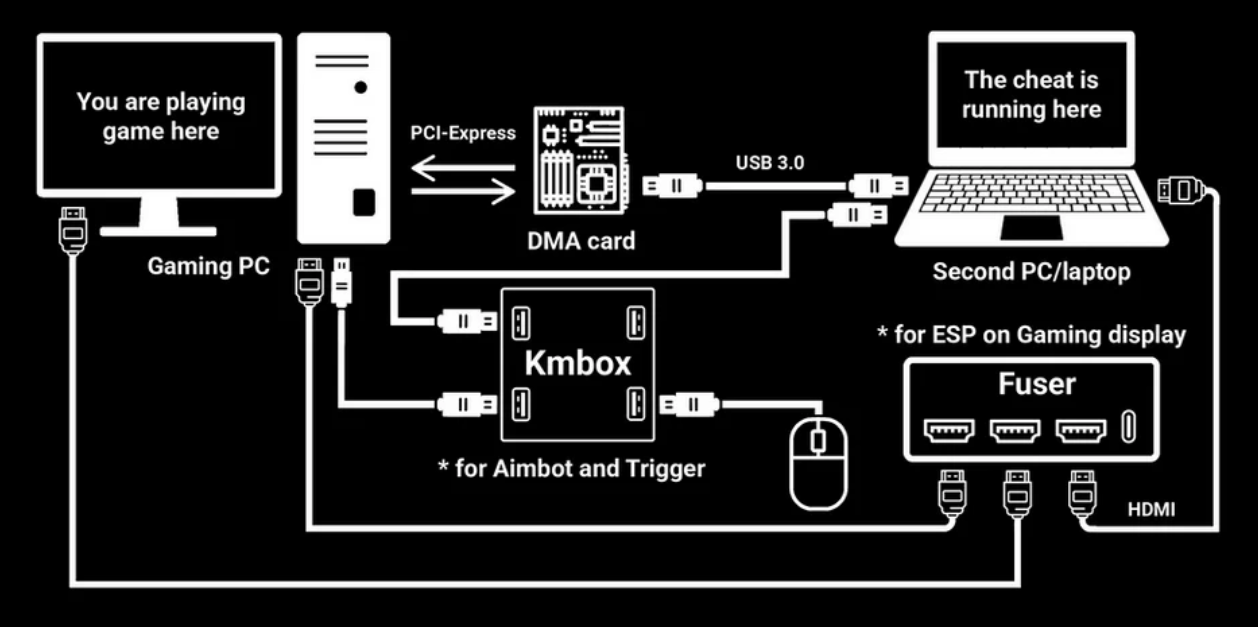
\includegraphics[height=7cm]{../images/chap01/fig5.png}
    \end{center}
    \caption[Infrastructure of a DMA cheat setup, where a specialized PCIe card reads the host system's RAM directly and transmits the data to an external machine for processing and input spoofing.]{https://steams360.com/blogs/news/what-are-dma-cheats-and-how-does-it-work}
    \label{fig:fig5}
\end{figure}

\section{Anti-Cheat Mechanisms}
\label{sec:one:two}

Faced with the escalating sophistication of cheating techniques described above, publishers have progressively layered three generations of countermeasures, each operating at a different level of system privilege and each responding to the specific evasion vectors that the previous generation could not address.

\subsection{Client-Side Anti-Cheats}
\label{sec:one:two:one}

Client-side anti-cheats operate within the same privilege boundary as the game itself — User Mode (Ring 3) — and rely primarily on two complementary techniques:

\begin{itemize}
    \item Code Injection Detection: these systems monitor the process for signs of external code being loaded into the game's memory space, such as unauthorized DLL injections or suspicious calls to process-manipulation functions. By maintaining a whitelist of legitimate modules and flagging any unexpected addition to the process's loaded module list, this technique targets the injection-based automation cheats described in Section 1.1.1.
    \item Memory Scanning: the anti-cheat periodically inspects the game process's memory space, comparing observed byte patterns against a database of known cheat signatures, or applying heuristic checks for anomalous memory regions (unexpected executable permissions, unusually allocated pages). This is conceptually the same operation performed manually in the experimental section of Chapter 2, where Cheat Engine is used to locate a specific value within process memory.
\end{itemize}

Empirical benchmarking of eleven competitive multiplayer titles confirms that the most technically robust client-side systems enforce a layered combination of file integrity checks, code injection countermeasures, and process scanning, and that the price of commercially available cheats correlates strongly with the measured sturdiness of the anti-cheat software they must bypass \cite{Collins2024}.

Because these mechanisms remain confined to Ring 3, however, they share the same fundamental blind spot as the user-mode game client itself: any cheat operating at a higher privilege level, or entirely outside the host process, falls outside their observable scope — the limitation that motivated the shift toward kernel-level solutions.

\subsection{Kernel-Level Anti-Cheats}
\label{sec:one:two:two}

Kernel-level anti-cheats close this visibility gap by operating at the same privilege level as the operating system itself — Ring 0 — mirroring the privilege escalation already adopted by advanced cheats (Section 1.1.3) and illustrated in Figure 4.

\begin{itemize}
    \item Privileged Monitoring: operating in Ring 0 grants the anti-cheat driver direct access to the full process list, raw physical and virtual memory, and low-level system structures, independently of any cooperation from the monitored process. This allows continuous observation of system state that a Ring 3 component could never access unfiltered.
    \item Detection of Low-Level Cheats: this elevated vantage point specifically targets the evasion techniques described in Section 1.1.3 — detecting the unauthorized loading of vulnerable drivers exploited via BYOVD, and identifying inconsistencies introduced by DKOM manipulation, such as a process artificially removed from the kernel's active process list but still consuming system resources elsewhere.
\end{itemize}

Yet formal analysis of these systems against rootkit classification criteria reveals that at least two of the four most widely deployed kernel-level solutions — FACEIT Anti-Cheat and Vanguard — satisfy a majority of the behavioral metrics used to characterize rootkits, including boot-time execution, binary virtualisation, and continuous system data exfiltration \cite{Dorner2024}. This structural resemblance between the very tool meant to protect the system and the threat model it defends against is a central tension that Chapter 2 examines in detail, and that Appendix D develops further from a privacy and regulatory perspective.

\subsection{Data-Driven Detection Methods}
\label{sec:one:two:three}

A third paradigm reframes the detection problem entirely by shifting the trust anchor away from the local machine and onto the game server, which — as the authoritative source of match state (Appendix C.1) — cannot be directly tampered with by the client.

\begin{itemize}
    \item Shifting the Trust Anchor: rather than inspecting the player's machine for evidence of cheat software, this approach analyzes the gameplay data the server already collects, reducing dependence on client-side integrity and enabling a global, cross-match view of player statistics unavailable to any single local process.
    \item Player Behavior Modeling: this data is used to characterize performance patterns, consistency across matches, and statistical deviations from expected human behavior — for instance, reaction times, aim precision, or decision-making patterns that fall outside the range observed in legitimate play.
\end{itemize}

Recent work demonstrates the concrete feasibility of this shift: a transformer-based model trained on kill-event context windows extracted from 795 labelled CS2 matches achieves an accuracy of 89\% and an AUC of 0.93 on an unaugmented test set, while maintaining a low false-positive rate — a requirement particularly critical in competitive contexts where erroneous bans carry direct reputational costs \cite{Loo2025}.

This approach, however, is not without conceptual limitations. Behavioral models remain exposed to false positives, particularly when distinguishing between a genuinely skilled player and a cheater exhibiting similarly consistent performance — a tension commonly referred to as the high-skill bias. Legitimate but statistically unusual play patterns (an exceptional clutch, an outlier reaction time) can likewise be misclassified as suspicious. These limitations are precisely what motivate the design choices explored in depth in Chapter 3.
